\documentclass{beamer}
\usetheme{Madrid}
\usecolortheme{dolphin}
\usepackage{tikz}
\usepackage{amsmath}
\usepackage{amssymb}

\title{Argument Evaluation}
\subtitle{Introduction to Logic}
\author{Professor's Name}
\date{\today}

\begin{document}

\begin{frame}
    \titlepage
\end{frame}

\begin{frame}{What is an Argument? Distinguishing Arguments from Other Forms of Discourse}
    \begin{itemize}
        \item An \textbf{argument} is a set of statements where some (the premises) are offered as support for another (the conclusion).
        \item Arguments differ from explanations, which tell why something happened rather than trying to prove it's true.
        \item Arguments differ from mere opinions, which don't offer reasoned support for claims.
        \item Arguments can be explicit (clearly stated) or implicit (with unstated assumptions).
    \end{itemize}
    
    \begin{alertblock}{Key Insight}
        Not all text containing claims is an argument—arguments specifically attempt to establish the truth of a conclusion through reasoning.
    \end{alertblock}
\end{frame}

\begin{frame}{The Building Blocks: Premises and Conclusions}
    \begin{itemize}
        \item \textbf{Premises} are the statements offered as reasons or evidence to support the conclusion.
        \item The \textbf{conclusion} is the statement that the premises are intended to establish or support.
        \item Every argument must have at least one premise and exactly one conclusion.
        \item The relationship between premises and conclusion constitutes the logical structure of the argument.
    \end{itemize}
    
    \begin{example}
        \textbf{Premise 1:} All humans are mortal.\\
        \textbf{Premise 2:} Socrates is human.\\
        \textbf{Conclusion:} Therefore, Socrates is mortal.
    \end{example}
\end{frame}

\begin{frame}{Indicator Words: How to Identify Premises and Conclusions}
    \begin{itemize}
        \item \textbf{Conclusion indicators} signal that a conclusion follows: "therefore," "thus," "hence," "so," "consequently."
        \item \textbf{Premise indicators} signal that a premise is being offered: "because," "since," "given that," "as."
        \item Indicator words provide clues but aren't always present in natural language arguments.
        \item Context often matters more than specific words when identifying premises and conclusions.
    \end{itemize}
    
    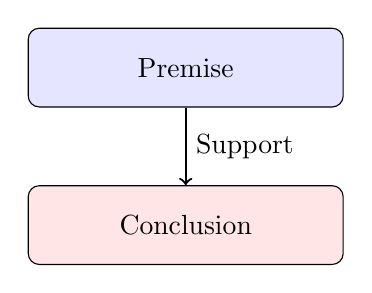
\begin{tikzpicture}
        \node[draw, rectangle, rounded corners, fill=blue!10, minimum width=4cm, minimum height=1cm] (premise) at (0,0) {Premise};
        \node[draw, rectangle, rounded corners, fill=red!10, minimum width=4cm, minimum height=1cm] (conclusion) at (0,-2) {Conclusion};
        \draw[->, thick] (premise) -- (conclusion) node[midway, right] {Support};
    \end{tikzpicture}
\end{frame}

\begin{frame}{Converting Arguments to Standard Form: A Step-by-Step Process}
    \begin{itemize}
        \item \textbf{Standard form} arranges an argument with premises listed first and the conclusion last.
        \item Step 1: Identify all statements that function as premises and the conclusion.
        \item Step 2: Eliminate irrelevant information and clarify ambiguous language.
        \item Step 3: Number the premises and label the conclusion for clear reference.
    \end{itemize}
    
    \begin{block}{Standard Form Template}
        Premise 1: [Statement]\\
        Premise 2: [Statement]\\
        $\vdots$\\
        Premise n: [Statement]\\
        Conclusion: [Statement]
    \end{block}
\end{frame}

\begin{frame}{Common Challenges in Identifying Arguments}
    \begin{itemize}
        \item Arguments in everyday language often contain \textbf{implicit premises} that must be reconstructed.
        \item Multiple conclusions may appear, requiring identification of the main conclusion.
        \item \textbf{Subarguments} occur when some premises are supported by other premises before supporting the main conclusion.
        \item Argumentative text is often mixed with rhetorical questions, examples, and repetition.
    \end{itemize}
    
    \begin{alertblock}{Warning}
        When reconstructing arguments, be careful not to create straw men by misrepresenting the original reasoning.
    \end{alertblock}
\end{frame}

\begin{frame}{The Dual Nature of Argument Evaluation}
    \begin{itemize}
        \item Argument evaluation requires answering two distinct questions about any argument.
        \item We must separate questions of \textbf{logical structure} from questions of \textbf{factual accuracy}.
        \item An argument can have a strong logical structure but false premises, or true premises but a weak structure.
        \item Complete evaluation requires examining both aspects independently before making a final judgment.
    \end{itemize}
    
    \begin{table}
        \centering
        \begin{tabular}{|c|c|c|}
            \hline
            & \textbf{True Premises} & \textbf{False Premises} \\
            \hline
            \textbf{Good Structure} & Strong argument & Weak argument \\
            \hline
            \textbf{Poor Structure} & Weak argument & Weak argument \\
            \hline
        \end{tabular}
        \caption{Argument strength depends on both structure and truth}
    \end{table}
\end{frame}

\begin{frame}{Question 1: Do the Premises Support the Conclusion? (Logical Structure)}
    \begin{itemize}
        \item This question examines the \textbf{inferential relationship} between premises and conclusion.
        \item We evaluate whether the premises provide good reasons to accept the conclusion, regardless of their truth.
        \item Different argument types have different standards for what counts as "good support."
        \item This evaluation focuses on form and pattern rather than content.
    \end{itemize}
    
    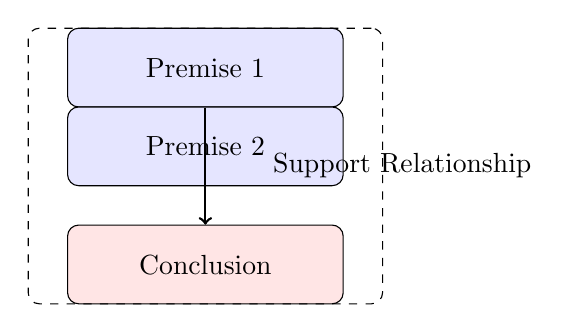
\begin{tikzpicture}
        \node[draw, rectangle, rounded corners, fill=blue!10, minimum width=3.5cm, minimum height=1cm] (p1) at (0,1) {Premise 1};
        \node[draw, rectangle, rounded corners, fill=blue!10, minimum width=3.5cm, minimum height=1cm] (p2) at (0,0) {Premise 2};
        \node[draw, rectangle, rounded corners, fill=red!10, minimum width=3.5cm, minimum height=1cm] (c) at (0,-1.5) {Conclusion};
        \draw[->, thick] (p1) -- (c);
        \draw[->, thick] (p2) -- (c);
        \node[draw, dashed, rectangle, rounded corners, minimum width=4.5cm, minimum height=3.5cm] at (0,-0.25) {};
        \node at (2.5,-0.25) {Support Relationship};
    \end{tikzpicture}
\end{frame}

\begin{frame}{Question 2: Are the Premises Actually True? (Factual Accuracy)}
    \begin{itemize}
        \item This question examines the \textbf{truth value} of each individual premise.
        \item Truth assessment requires domain knowledge beyond pure logic.
        \item Premises may be certainly true, certainly false, or somewhere in between.
        \item For complex arguments, we should assess the likelihood of each premise independently.
    \end{itemize}
    
    \begin{exampleblock}{Methods for Assessing Truth}
        \begin{itemize}
            \item Direct observation
            \item Expert testimony
            \item Statistical evidence
            \item Established scientific knowledge
        \end{itemize}
    \end{exampleblock}
\end{frame}

\begin{frame}{The Relationship Between Structure and Truth}
    \begin{itemize}
        \item An argument with true premises but poor structure gives no good reason to accept the conclusion.
        \item An argument with excellent structure but false premises cannot establish a true conclusion.
        \item The strongest arguments combine true premises with strong logical structure.
        \item \textbf{Formal fallacies} occur in the structure, while \textbf{informal fallacies} often involve questionable premises.
    \end{itemize}
    
    \begin{block}{The Logic Formula}
        Good argument = Valid/Strong structure + True premises
    \end{block}
\end{frame}

\begin{frame}{Three Major Categories of Arguments: An Overview}
    \begin{itemize}
        \item Arguments can be classified into three major types based on the relationship claimed between premises and conclusion.
        \item Each type of argument makes a different kind of claim about how strongly its premises support its conclusion.
        \item The type of argument determines the appropriate standards for evaluating its logical structure.
        \item Recognizing argument type is the first step in proper evaluation.
    \end{itemize}
    
    \begin{table}
        \centering
        \begin{tabular}{|l|l|l|}
            \hline
            \textbf{Argument Type} & \textbf{Claimed Support} & \textbf{Evaluation Terms} \\
            \hline
            Deductive & Necessity & Valid/Invalid \\
            \hline
            Inductive & Probability & Strong/Weak \\
            \hline
            Abductive & Best Explanation & Better/Worse \\
            \hline
        \end{tabular}
    \end{table}
\end{frame}

\begin{frame}{Deductive Arguments: Claiming Necessity}
    \begin{itemize}
        \item \textbf{Deductive arguments} claim that if their premises are true, their conclusion must necessarily be true.
        \item They aim for certainty based on the logical form of the argument.
        \item Deductive reasoning moves from general principles to specific conclusions.
        \item Common forms include syllogisms, modus ponens, modus tollens, and mathematical proofs.
    \end{itemize}
    
    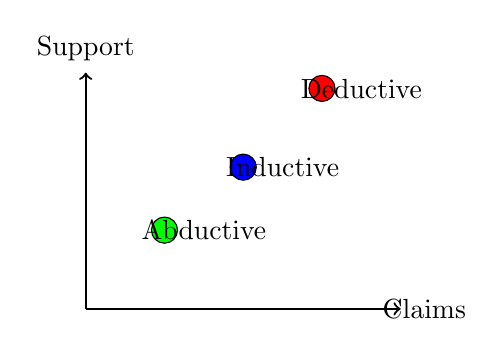
\begin{tikzpicture}
        \draw[thick, ->] (0,0) -- (4,0);
        \draw[thick, ->] (0,0) -- (0,3);
        \node at (4.3,0) {Claims};
        \node at (0,3.3) {Support};
        \node[circle, fill=red, draw, minimum size=0.2cm] at (3,2.8) {};
        \node at (3.5,2.8) {Deductive};
        \node[circle, fill=blue, draw, minimum size=0.2cm] at (2,1.8) {};
        \node at (2.5,1.8) {Inductive};
        \node[circle, fill=green, draw, minimum size=0.2cm] at (1,1) {};
        \node at (1.5,1) {Abductive};
    \end{tikzpicture}
\end{frame}

\begin{frame}{Inductive Arguments: Claiming Probability}
    \begin{itemize}
        \item \textbf{Inductive arguments} claim that if their premises are true, their conclusion is probably true.
        \item They aim for likelihood rather than certainty, allowing for exceptions.
        \item Inductive reasoning typically moves from specific observations to general conclusions.
        \item Common forms include generalizations, statistical arguments, and analogical reasoning.
    \end{itemize}
    
    \begin{exampleblock}{Inductive Example}
        Premise 1: Swan 1 is white.\\
        Premise 2: Swan 2 is white.\\
        Premise 3: Swan 3 is white.\\
        $\vdots$\\
        Premise 100: Swan 100 is white.\\
        Conclusion: Probably, all swans are white.
    \end{exampleblock}
\end{frame}

\begin{frame}{Abductive Arguments: Seeking the Best Explanation}
    \begin{itemize}
        \item \textbf{Abductive arguments} claim that their conclusion is the best explanation for the evidence presented in the premises.
        \item They aim to identify the most plausible cause or reason among competing hypotheses.
        \item Abductive reasoning moves from observations to likely explanations.
        \item Common in scientific discovery, medical diagnosis, and detective work.
    \end{itemize}
    
    \begin{block}{Characteristics of Good Explanations}
        \begin{itemize}
            \item Simplicity (Occam's Razor)
            \item Explanatory scope
            \item Consistency with background knowledge
            \item Lack of ad hoc elements
        \end{itemize}
    \end{block}
\end{frame}

\begin{frame}{Clues for Identifying Argument Types in Natural Language}
    \begin{itemize}
        \item Deductive arguments often use terms like "necessarily," "certainly," "must be," or "it follows that."
        \item Inductive arguments often use terms like "probably," "likely," "tends to," or "in most cases."
        \item Abductive arguments often use terms like "best explains," "most reasonable account," or "most plausible reason."
        \item Context and content also provide clues about the intended argument type.
    \end{itemize}
    
    \begin{table}
        \centering
        \begin{tabular}{|l|l|}
            \hline
            \textbf{Language Used} & \textbf{Likely Argument Type} \\
            \hline
            "All X are Y" & Deductive \\
            "Most X are Y" & Inductive \\
            "The evidence suggests..." & Inductive or Abductive \\
            "This would explain why..." & Abductive \\
            \hline
        \end{tabular}
    \end{table}
\end{frame}

\begin{frame}{Practice: Classifying Arguments by Type}
    \begin{itemize}
        \item Identifying argument type is a skill that improves with practice.
        \item Consider both the language used and the intended strength of the conclusion.
        \item Arguments may combine elements of different types or be ambiguous.
        \item When in doubt, consider what standards the arguer would accept as appropriate for evaluation.
    \end{itemize}
    
    \begin{alertblock}{Common Mistake}
        Don't confuse the actual strength of an argument with its intended type. A weak deductive argument is still deductive in type, even if it fails to establish necessity.
    \end{alertblock}
\end{frame}

\begin{frame}{The Ideal of Deductive Reasoning: Guaranteeing Truth Preservation}
    \begin{itemize}
        \item Deductive reasoning aims to \textbf{preserve truth} from premises to conclusion.
        \item If the premises are true and the reasoning is valid, the conclusion must be true.
        \item Truth preservation is binary: either an argument preserves truth or it doesn't.
        \item This provides certainty but requires meeting a high standard of evidence and reasoning.
    \end{itemize}
    
    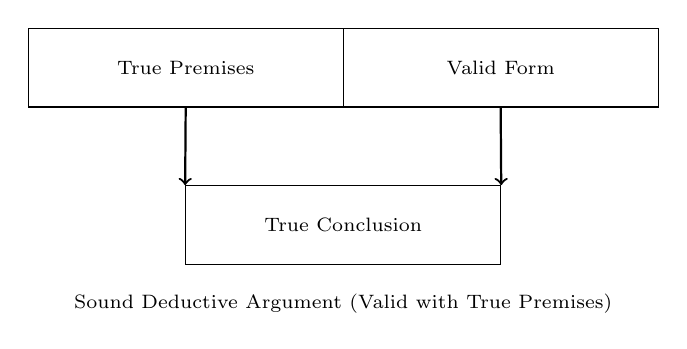
\begin{tikzpicture}
        \scriptsize
        \node[draw, rectangle, minimum width=4cm, minimum height=1cm] (premises) at (-2,0) {True Premises};
        \node[draw, rectangle, minimum width=4cm, minimum height=1cm] (valid) at (2,0) {Valid Form};
        \node[draw, rectangle, minimum width=4cm, minimum height=1cm] (conclusion) at (0,-2) {True Conclusion};
        \draw[thick, ->] (premises.south) -- (conclusion.north west);
        \draw[thick, ->] (valid.south) -- (conclusion.north east);
        \node at (0,-3) {Sound Deductive Argument (Valid with True Premises)};
    \end{tikzpicture}
\end{frame}

\begin{frame}{Validity: What It Means and What It Doesn't}
    \begin{itemize}
        \item An argument is \textbf{valid} if and only if it's impossible for its premises to be true while its conclusion is false.
        \item Validity is about the logical structure of the argument, not about the truth of its premises.
        \item A valid argument with false premises can lead to a false conclusion.
        \item Validity doesn't guarantee truth—it guarantees that truth flows from premises to conclusion if the premises are true.
    \end{itemize}
    
    \begin{exampleblock}{Valid Argument with False Premises}
        Premise 1: All lizards have six legs.\\
        Premise 2: Komodo dragons are lizards.\\
        Conclusion: Therefore, Komodo dragons have six legs.\\
        
        \textit{This argument is valid but unsound because Premise 1 is false.}
    \end{exampleblock}
\end{frame}

\begin{frame}{Counterexamples: The Power of a Single Case}
    \begin{itemize}
        \item A \textbf{counterexample} is a scenario where the premises are true but the conclusion is false.
        \item Finding even one counterexample proves an argument is invalid.
        \item Counterexamples show that the logical form of the argument allows for exceptions.
        \item Constructing counterexamples is one of the most powerful tools for evaluating deductive arguments.
    \end{itemize}
    
    \begin{alertblock}{How to Construct a Counterexample}
        1. Accept all premises as true (for the sake of argument)\\
        2. Imagine a situation where the conclusion is false\\
        3. Verify that this situation doesn't contradict any premises\\
        4. If successful, you've found a counterexample
    \end{alertblock}
\end{frame}

\begin{frame}{Finding Counterexamples: Systematic Strategies}
    \begin{itemize}
        \item Replace terms in the argument with variables, then find substitutions that invalidate it.
        \item Consider extreme or boundary cases that satisfy the premises but not the conclusion.
        \item Use analogical reasoning to construct parallel arguments with obviously false conclusions.
        \item For categorical arguments, use Venn diagrams to find possible counterexamples.
    \end{itemize}
    
    \begin{example}
        Original: "All doctors are educated. Sarah is educated. Therefore, Sarah is a doctor."\\
        
        Counterexample structure: "All A are B. C is B. Therefore, C is A."\\
        
        Substitute: "All dogs are mammals. Cats are mammals. Therefore, cats are dogs."\\
        
        This shows the original argument form is invalid.
    \end{example}
\end{frame}

\begin{frame}{Formal Methods of Argument Evaluation: Logic Systems and Rules}
    \begin{itemize}
        \item \textbf{Formal logic} provides systematic methods for evaluating deductive arguments.
        \item Propositional logic uses truth tables to test validity by examining all possible truth value combinations.
        \item Predicate logic uses quantifiers and relations to analyze more complex arguments.
        \item Rule-based systems employ rules of inference like modus ponens and modus tollens.
    \end{itemize}
    
    \begin{block}{Basic Rules of Inference}
        \textbf{Modus Ponens:} If P → Q and P, then Q\\
        \textbf{Modus Tollens:} If P → Q and not Q, then not P\\
        \textbf{Hypothetical Syllogism:} If P → Q and Q → R, then P → R\\
        \textbf{Disjunctive Syllogism:} If P or Q and not P, then Q
    \end{block}
\end{frame}

\begin{frame}{Soundness: When Valid Arguments Have True Premises}
    \begin{itemize}
        \item A deductive argument is \textbf{sound} if and only if it is valid and all its premises are true.
        \item Soundness is the gold standard for deductive arguments—it guarantees a true conclusion.
        \item An argument can be valid but unsound if any of its premises are false.
        \item Soundness requires both logical and factual evaluation.
    \end{itemize}
    
    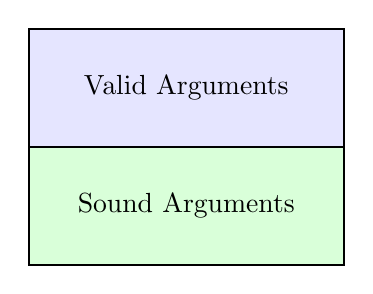
\begin{tikzpicture}
        \fill[blue!10] (0,0) rectangle (4,3);
        \fill[green!15] (0,0) rectangle (4,1.5);
        \node at (2,2.25) {Valid Arguments};
        \node at (2,0.75) {Sound Arguments};
        \draw[thick] (0,0) rectangle (4,3);
        \draw[thick] (0,1.5) -- (4,1.5);
    \end{tikzpicture}
\end{frame}

\begin{frame}{The Nature of Inductive Strength: Degrees of Support}
    \begin{itemize}
        \item Unlike validity, \textbf{inductive strength} is a matter of degree rather than all-or-nothing.
        \item An inductively strong argument makes its conclusion probable but not certain.
        \item The strength of an inductive argument increases with more relevant evidence.
        \item Inductive arguments can be undermined by new evidence without being completely defeated.
    \end{itemize}
    
    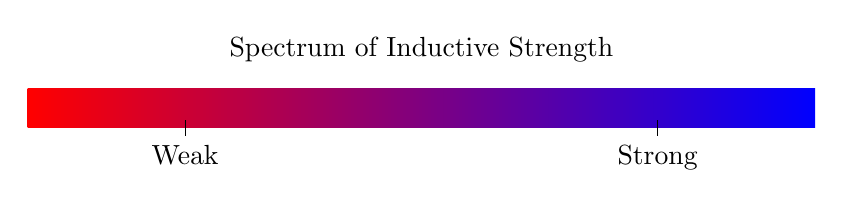
\begin{tikzpicture}
        \node at (5,1) {Spectrum of Inductive Strength};
        \shade[left color=red, right color=blue] (0,0) rectangle (10,0.5);
        \draw (2,0.1) -- (2,-0.1) node[below] {Weak};
        \draw (8,0.1) -- (8,-0.1) node[below] {Strong};
    \end{tikzpicture}
\end{frame}

\begin{frame}{Evaluating Sample Size: When Is Evidence Sufficient?}
    \begin{itemize}
        \item The \textbf{sample size} of an inductive argument directly affects its strength.
        \item Larger samples generally provide stronger support for generalizations.
        \item The required sample size depends on the population variability and claim specificity.
        \item Sample size requirements increase when making precise or counter-intuitive claims.
    \end{itemize}
    
    \begin{table}
        \centering
        \begin{tabular}{|l|c|c|}
            \hline
            \textbf{Claim Type} & \textbf{Small Sample} & \textbf{Large Sample} \\
            \hline
            General trend & Weak support & Strong support \\
            \hline
            Precise percentage & Very weak & Moderate support \\
            \hline
            Universal claim & Extremely weak & Moderate support \\
            \hline
        \end{tabular}
    \end{table}
\end{frame}

\begin{frame}{Representative Samples: Quality Matters as Much as Quantity}
    \begin{itemize}
        \item A \textbf{representative sample} accurately reflects the relevant characteristics of the whole population.
        \item Biased sampling can lead to false generalizations even with large sample sizes.
        \item Common biases include selection bias, volunteer bias, and confirmation bias.
        \item Random sampling helps ensure representativeness but doesn't guarantee it.
    \end{itemize}
    
    \begin{alertblock}{Warning Signs of Poor Samples}
        \begin{itemize}
            \item Sample drawn from a convenience population
            \item Self-selected participants
            \item Narrow demographic representation
            \item High dropout or non-response rates
        \end{itemize}
    \end{alertblock}
\end{frame}

\begin{frame}{Cogency: The Inductive Counterpart to Soundness}
    \begin{itemize}
        \item An inductive argument is \textbf{cogent} if it is strong and all its premises are true.
        \item Cogency is to inductive arguments what soundness is to deductive arguments.
        \item A cogent argument provides good but not conclusive reasons to accept its conclusion.
        \item Even cogent arguments may be overturned by new evidence.
    \end{itemize}
    
    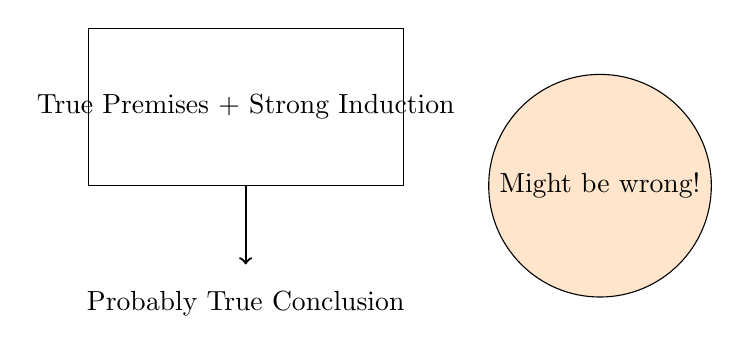
\begin{tikzpicture}
        \draw (0,0) rectangle (4,2);
        \draw[thick, ->] (2,0) -- (2,-1);
        \node at (2,1) {True Premises + Strong Induction};
        \node at (2,-1.5) {Probably True Conclusion};
        \node[draw, circle, fill=orange!20] at (6.5,0) {Might be wrong!};
    \end{tikzpicture}
\end{frame}

\begin{frame}{Inductive Generalizations vs. Statistical Syllogisms}
    \begin{itemize}
        \item \textbf{Inductive generalizations} move from observed instances to a general claim about a class (Some → All).
        \item \textbf{Statistical syllogisms} move from a general statistical claim to a prediction about a specific case (All → Some).
        \item Both forms depend on sample representativeness but in different ways.
        \item Potential fallacies differ depending on the direction of inference.
    \end{itemize}
    
    \begin{exampleblock}{Two Directions of Inductive Reasoning}
        \textbf{Generalization:} "80\% of observed swans were white, so approximately 80\% of all swans are white."
        
        \textbf{Statistical Syllogism:} "Approximately 80\% of swans are white, so this particular swan is probably white."
    \end{exampleblock}
\end{frame}

\begin{frame}{Common Inductive Fallacies and How to Avoid Them}
    \begin{itemize}
        \item The \textbf{hasty generalization} fallacy occurs when conclusions are drawn from too few examples.
        \item The \textbf{biased sample} fallacy occurs when evidence is not representative of the population.
        \item The \textbf{gambler's fallacy} incorrectly assumes that past random events influence future ones.
        \item The \textbf{appeal to anecdote} fallacy treats personal stories as statistically significant evidence.
    \end{itemize}
    
    \begin{block}{Preventing Inductive Fallacies}
        \begin{itemize}
            \item Ensure adequate sample size
            \item Check for sample representativeness
            \item Look for potential confounding variables
            \item Consider alternative explanations
        \end{itemize}
    \end{block}
\end{frame}

\begin{frame}{The Logic of Explanation: What Makes an Explanation Good?}
    \begin{itemize}
        \item \textbf{Abductive reasoning} seeks the best explanation for a set of observations or facts.
        \item Good explanations must account for the evidence more effectively than alternatives.
        \item Abductive arguments compare competing hypotheses rather than testing a single hypothesis.
        \item The "best explanation" is judged according to multiple criteria, not just one.
    \end{itemize}
    
    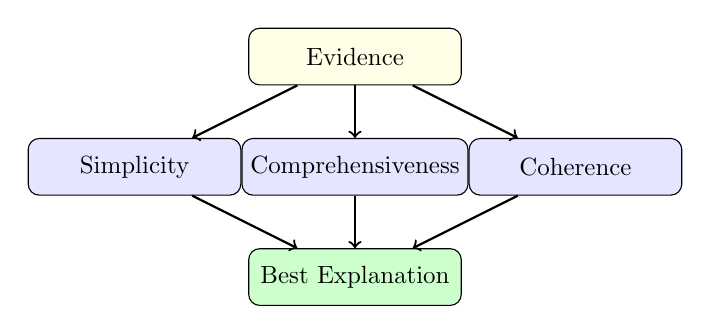
\begin{tikzpicture}[scale=0.7, every node/.style={scale=0.9}]
        \node[draw, rectangle, rounded corners, fill=yellow!10, minimum width=3cm, minimum height=0.8cm] (evidence) at (0,0) {Evidence};
        \node[draw, rectangle, rounded corners, fill=blue!10, minimum width=3cm, minimum height=0.8cm] (simplicity) at (-4,-2) {Simplicity};
        \node[draw, rectangle, rounded corners, fill=blue!10, minimum width=3cm, minimum height=0.8cm] (comprehensiveness) at (0,-2) {Comprehensiveness};
        \node[draw, rectangle, rounded corners, fill=blue!10, minimum width=3cm, minimum height=0.8cm] (coherence) at (4,-2) {Coherence};
        \node[draw, rectangle, rounded corners, fill=green!20, minimum width=3cm, minimum height=0.8cm] (best) at (0,-4) {Best Explanation};
        \draw[->, thick] (evidence) -- (simplicity);
        \draw[->, thick] (evidence) -- (comprehensiveness);
        \draw[->, thick] (evidence) -- (coherence);
        \draw[->, thick] (simplicity) -- (best);
        \draw[->, thick] (comprehensiveness) -- (best);
        \draw[->, thick] (coherence) -- (best);
    \end{tikzpicture}
\end{frame}

\begin{frame}{Criteria for Evaluating Explanations: Simplicity}
    \begin{itemize}
        \item \textbf{Simplicity} (also called parsimony) favors explanations that make fewer assumptions.
        \item Occam's Razor states that we should not multiply entities beyond necessity.
        \item Simpler explanations are less likely to include false assumptions.
        \item Simplicity must be balanced against explanatory power—overly simple explanations may miss important factors.
    \end{itemize}
    
    \begin{exampleblock}{Balancing Simplicity and Explanatory Power}
        Consider two explanations for a patient's symptoms:
        
        Explanation 1: The patient has one common disease that explains most symptoms.
        
        Explanation 2: The patient has three rare diseases that collectively explain all symptoms.
        
        Unless Explanation 1 fails to account for critical symptoms, it is preferable due to its simplicity.
    \end{exampleblock}
\end{frame}

\begin{frame}{Criteria for Evaluating Explanations: Comprehensiveness}
    \begin{itemize}
        \item \textbf{Comprehensiveness} refers to how much of the evidence an explanation accounts for.
        \item A good explanation should explain all or most of the relevant facts.
        \item Unexplained anomalies weaken an explanation's plausibility.
        \item Explanations that need frequent modifications to accommodate new evidence are suspect.
    \end{itemize}
    
    \begin{block}{Comprehensive vs. Selective Explanations}
        \begin{itemize}
            \item Comprehensive: Explains all the evidence
            \item Moderately comprehensive: Explains most key evidence
            \item Selective: Cherry-picks favorable evidence
            \item Ad hoc: Requires different mechanisms for each piece of evidence
        \end{itemize}
    \end{block}
\end{frame}

\begin{frame}{Criteria for Evaluating Explanations: Coherence with Background Knowledge}
    \begin{itemize}
        \item Good explanations should be \textbf{consistent} with well-established theories and facts.
        \item Extraordinary claims require extraordinary evidence.
        \item Background knowledge provides a prior probability for competing explanations.
        \item Coherence measures how well an explanation fits with our broader understanding.
    \end{itemize}
    
    \begin{alertblock}{Weighing Coherence Against Evidence}
        When evidence strongly suggests an explanation that conflicts with background knowledge, we face three options:
        \begin{itemize}
            \item Question the reliability of the new evidence
            \item Revise our background knowledge
            \item Seek a third explanation that reconciles both
        \end{itemize}
    \end{alertblock}
\end{frame}

\begin{frame}{The Problem of Alternative Explanations}
    \begin{itemize}
        \item Abductive reasoning is limited by our ability to generate alternative explanations.
        \item The "best explanation" is only the best among those we've considered.
        \item \textbf{Underconsideration} occurs when we fail to consider a wide enough range of hypotheses.
        \item Strong abductive arguments explicitly address and eliminate viable alternatives.
    \end{itemize}
    
    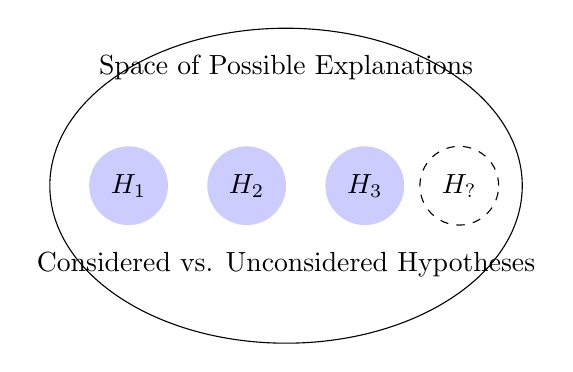
\begin{tikzpicture}
        \draw (0,0) ellipse (3cm and 2cm);
        \node at (0,1.5) {Space of Possible Explanations};
        \fill[blue!20] (-2,0) circle (0.5cm);
        \fill[blue!20] (-0.5,0) circle (0.5cm);
        \fill[blue!20] (1,0) circle (0.5cm);
        \node at (-2,0) {$H_1$};
        \node at (-0.5,0) {$H_2$};
        \node at (1,0) {$H_3$};
        \draw[dashed] (2.2,0) circle (0.5cm);
        \node at (2.2,0) {$H_?$};
        \node at (0,-1) {Considered vs. Unconsidered Hypotheses};
    \end{tikzpicture}
\end{frame}

\begin{frame}{Uniting the Methods: Choosing the Right Evaluation Strategy}
    \begin{itemize}
        \item Different argument types require different evaluation methods.
        \item Deductive arguments should be evaluated for validity and soundness.
        \item Inductive arguments should be evaluated for strength and cogency.
        \item Abductive arguments should be evaluated by comparing the quality of competing explanations.
    \end{itemize}
    
    \begin{table}
        \scriptsize
        \centering
        \begin{tabular}{|l|l|l|}
            \hline
            \textbf{If the argument is...} & \textbf{Ask these questions...} & \textbf{Using these methods...} \\
            \hline
            Deductive & Is it valid? Are premises true? & Counterexamples, formal logic \\
            \hline
            Inductive & Is it strong? Are premises true? & Sample analysis, verification \\
            \hline
            Abductive & Is it the best explanation? & Comparative hypothesis testing \\
            \hline
        \end{tabular}
    \end{table}
\end{frame}

\begin{frame}{Common Mistakes in Argument Evaluation}
    \begin{itemize}
        \item Evaluating an argument using criteria meant for a different argument type.
        \item Focusing only on structure without verifying premises (or vice versa).
        \item Dismissing an argument due to minor flaws rather than evaluating its core reasoning.
        \item Accepting an argument based on agreeing with its conclusion rather than its logic.
    \end{itemize}
    
    \begin{exampleblock}{Evaluation Mistake Example}
        Criticizing an inductive argument for not being deductively valid:
        
        "This argument about climate patterns based on decades of data isn't valid because there could theoretically be exceptions."
        
        This misapplies deductive standards to an inductive argument.
    \end{exampleblock}
\end{frame}

\begin{frame}{Summary: The Complete Toolkit for Argument Evaluation}
    \begin{itemize}
        \item Begin by identifying the argument type: deductive, inductive, or abductive.
        \item Evaluate the logical structure according to the appropriate standards for that type.
        \item Independently verify the truth or acceptability of the premises.
        \item Consider the argument as a whole—is it valid/strong AND sound/cogent?
    \end{itemize}
    
    \begin{block}{The Critical Thinker's Checklist}
        \begin{enumerate}
            \item Reconstruct the argument in standard form
            \item Identify the argument type
            \item Evaluate logical structure (validity/strength/best explanation)
            \item Assess premise truth
            \item Deliver verdict on overall argument quality
        \end{enumerate}
    \end{block}
\end{frame}

\end{document}